\documentclass[a4paper,11pt]{article}

\usepackage[margin=3cm]{geometry}

\usepackage{graphicx}
\usepackage{subcaption}
\usepackage[colorlinks,allcolors=violet]{hyperref}
\usepackage{url}

% https://tex.stackexchange.com/questions/94032/fancy-tables-in-latex
\usepackage[table]{xcolor}
\usepackage{booktabs}

\usepackage[utf8]{inputenc}

% https://tex.stackexchange.com/questions/664/why-should-i-use-usepackaget1fontenc
\usepackage[T1]{fontenc}


\newcommand{\note}[1]{{\colorbox{yellow!40!white}{#1}}}
\newcommand{\exampletext}[1]{{\color{blue!60!black}#1}}

\begin{document}

\noindent
\colorbox[HTML]{52BDEC}{\bfseries\parbox{\textwidth}{\centering\large
  --- Code review P\&O CW 2019--2020 Task ID2 ---
}}
\\[-1mm]
\colorbox[HTML]{00407A}{\bfseries\color{white}\parbox{\textwidth}{
  Department of Computer Science -- KU Leuven
  \hfill
  \today
}}
\\

\smallskip

\noindent
%\mbox{}\hfill
\begin{tabular}{*4l}
\toprule
\multicolumn{3}{l}{\large\textbf{Team 12}} \\
\midrule
Toon Sauvillers & 2h & 270 LOC \\ % fill in the time spend on this task per team member who worked on it and the amount of lines of code (LOC) reviewed
Bert Van den Bosch & 2h & 389 LOC \\
\bottomrule
\hline
\end{tabular}\\
\\
Files reviewed: RGBBarcodeScanner.js; PixelIterator.js; Animation.js	

\noindent
{\color[HTML]{52BDEC} \rule{\linewidth}{1mm} }

\smallskip
\section{Inleiding}
Het tweede semester begon met het verbeteren van ons project. In ons geval was dit vooral de barcodescanner en de animatie(synchronisatie) die zich aan een opknapbeurt mochten verwachten. De rest van het project hebben we ongeschonden gelaten, niet omdat dit perfecte code is. Het is code die momenteel werkt en dat vinden we het belangrijkste. Echter zijn er nog veel stijlopmerkingen hierover te maken en aangezien dit enkel stijlopmerkingen zijn en deze hetzelfde zijn als vorig semester, laten we deze buiten beschouwing in dit verslag.

Deze codereview behandeld de twee componenten die verbetert zijn, mede door de bekomen resultaten te gebruiken van de testen in het begin van het semester. De animatie(synchronisatie) werd behandeld door Bert en de barcodescanner door Toon.

\section{RGBBarcodeScanner.js}
\begin{itemize}
	\item Om de gehele afbeelding te scannen wordt er gebruik gemaakt van een iterator. Dit is een goede keuze om een {\it nulpointer exception} te vermijden. Het wordt gebruikt om, ook al staat het scherm niet gelijk met de afbeelding, toch het scherm van links naar rechts horizontaal te overlopen. Het in een iterator te schrijven vergroot de leesbaarheid en correctheid.
	\item Voor het filteren van noise wordt er gebruikt gemaakt van een while loop om elke rij (volgens de iterator) apart te filteren. Zie figuur \ref{startFilter} Duidelijker zou zijn dat de foto in zijn geheel wordt gefilterd in een aparte functie. Deze functie zou dan deze while lus bevatten.
	\item Vervolgens wordt in de noiseFilter voor elke rij dezelfde bewerking gedaan, met dezelfde gegevens van het spectrum. Zie figuur \ref{noiseFilter}. Aangezien het spectrum steeds hetzelfde is, kunnen deze bewerkingen éénmalig worden gedaan en worden meegegeven.
	\item Ook in de while-lus in figuur \ref{startFilter} wordt er gekeken naar de barcodes per rij. Dit lijkt ook beter en duidelijker moest er eerst gefilterd worden en vervolgens, in een aparte lus, gescanned worden op barcodes. Deze verandering maakt het ook mogelijk om in de toekomst gemakkelijker aanpassingen te doen voor het filteren en het scannen van barcodes apart.
	\item In scanRow, waar de barcodes worden gescand, wordt heel vaak $ value/255$ gedaan. Dit is echter redundant, het oogt mooier doordat je later kan checken op $==1$, waarden zijn namelijk of 0 of 255. Als men echter controleert op $==255$ moet men niet steeds hierdoor delen.
	\item Voor het vinden van het procentueel aantal juiste barcodes wordt er gebruikt gemaakt van lambdafuncties. Dit oogt zeer mooi en overzichtelijk! Zie figuur \ref{lambda}. Hier zou echter wel mogen bijstaan in de comments om dit eventueel weg te halen. Het wordt nu enkel gebruikt om te loggen.
	\item Ook voor {\it getHighestCode} wordt er ook gebruikt gemaakt van een lambdafunctie. Zie figuur \ref{getHighestCode}
\end{itemize}

\begin{figure}
	\centering
	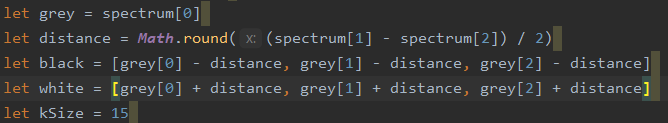
\includegraphics{img/noiseFilter}
	\caption{Deel van de noiseFilter die voor elke lijn herhaald wordt.}
	\label{noiseFilter}
\end{figure}

\begin{figure}
	\centering
	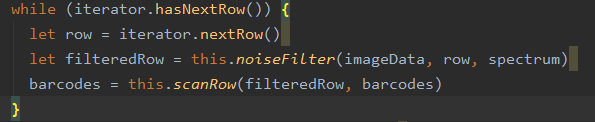
\includegraphics{img/startFilter}
	\caption{While-lus in de scan functie}
	\label{startFilter}
\end{figure}
\begin{figure}
	\centering
	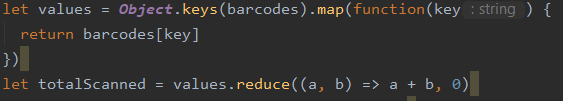
\includegraphics{img/lambda}
	\caption{Lambda functies om de juiste code te vinden.}
	\label{lambda}
\end{figure}
\begin{figure}
	\centering
	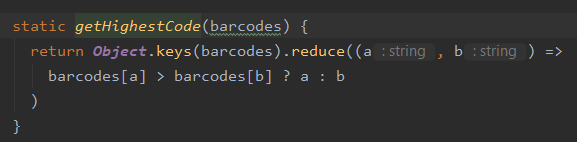
\includegraphics{img/getHighestCode}
	\caption{Lambdafuncties in {\it getHighestCode}}
	\label{getHighestCode}
\end{figure}

\section{Animation.js}

\begin{itemize}
	\item Over de triangulatie van de verschillende schermen lopen dieren achter elkaar om de synchrone animatie over de verschillende schermen te tonen. Dit was deel van de opdracht van het eerste semester, maar werd geüpdatet in het begin van dit semester.
	
	\item Over het algemeen mist de gehele klasse documentatie. Van de instructor tot grote methodes. Enkele functies zijn van zelfsprekend, maar het grotendeel is het voor een gebruiker dat de code nog nooit heeft gezien een gokwerk van de verschillende parameters en resultaat van de functie in kwestie.
	
	\item De functie $go(dx, dy)$ gebruikt twee function calls om eerst verticaal te verplaatsen en vervolgens horizontaal. Dit oogt mooi, maar is niet efficiënt aangezien deze methodes om volgens de x- en respectievelijke y-as te transleren enkel door de algemene $go()$ functie worden opgeroepen. Dit maakt dat deze extra methodes redundant zijn en de algemen functie efficiënter kan door de volledige translatie in één keer uit te voeren. (Zie figuur \ref{go}.)
	
	\item De code om de verschillende dieren af te beelden is niet voorbedachte raden geschreven op uitbreiding. De afbeelding van de twee gebruikte dieren worden geïnitialiseerd in de constructor. Beide dieren hebben een standaard en een kerst versie. Voor twee dieren gaat dit nog net in de constructor, maar de verschillende $if-statements$ maken de constructor onnodig lang. Deze initialisatie zou zich beter in een eigen methode bevinden om de constructor niet storend lang te maken bij het toevoegen van meerdere dieren.\\
	Ook de methode $drawAnimal()$ is nu gebaseerd op een boolean van welk dier er getekend moet worden en heeft dus een herschrijving nodig om meer dan twee dieren aan te kunnen. (Zie afbeelding \ref{boolAnimal}.)\\
	Om de verschillende dieren hun frame te updaten wordt er nu een groot deel code twee maal met maar een minimale aanpassing gebruikt in $drawAnimals()$. Ook hier kan er gerefactord worden om meerdere dieren aan te kunnen zonder dat er veel aangepast moet worden en repetitieve code te vermijden. (Zie afbeelding \ref{repetitive}.)
	
	\item De volledige klasse kan ook een opkuis gebruiken. Er zijn hier en daar nog overtollige $console.log$ restanten van het debuggen, volledig gecommentarieerde functies en redundante parameters in een methode
\end{itemize}

\begin{figure}
	\centering
	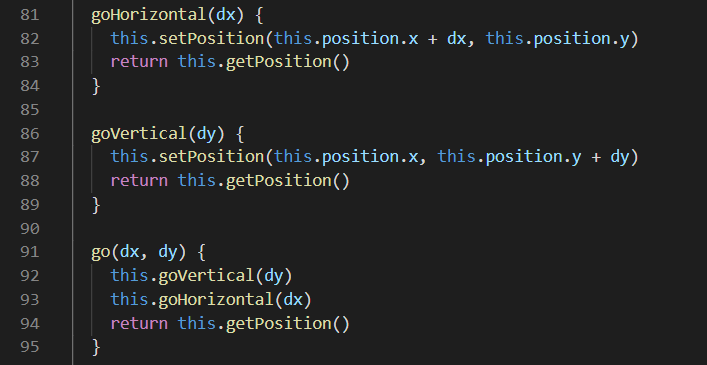
\includegraphics{img/go.png}
	\caption{Redundate methodes voor translatie.}
	\label{go}
\end{figure}

\begin{figure}
	\centering
	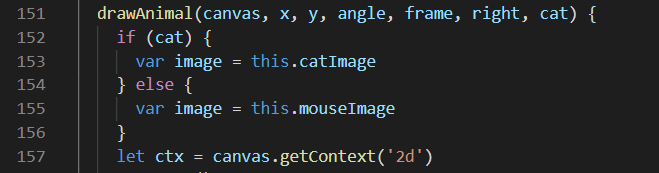
\includegraphics{img/animals.png}
	\caption{Maar twee soorten dieren supported door gebruik van boolean als parameter.}
	\label{boolAnimal}
\end{figure}

\begin{figure}
	\centering
	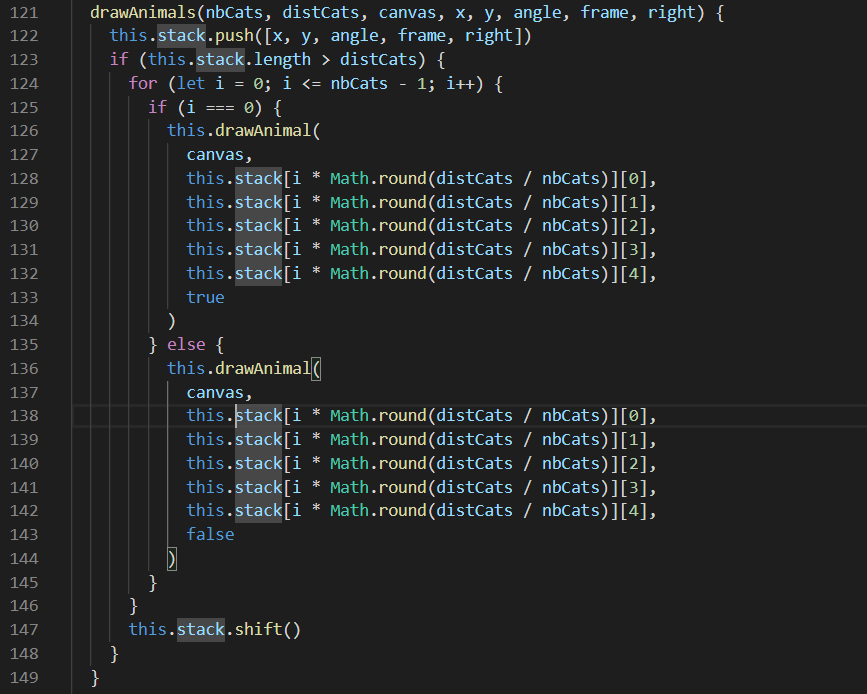
\includegraphics{img/repetitive.png}
	\caption{Repetitieve code.}
	\label{repetitive}
\end{figure}

\section{Besluit}
Er zijn nog enkele opmerkingen gevonden. Zowel qua stijl, performantie en documentatie kan er nog wat verbeterd worden. Vooral de performantie hopen we zeker nog aan te pakken, al is deze met de nieuwe code al sterk verbeterd ten opzichte van vorig semester. We wouden nog afsluiten met een mopje maar onze teamgenoten vonden dit niet grappig, dit besparen we jullie dan ook.

\end{document}